\section{Handling the path}

The most important factor in developing a processing package is handling the path. In each step of programming, we need to know, where we are, and where we want to be (in terms of computer path). Where is the input data and where we need to print out the output data. We accept the following axioms:

\begin{itemize}
  \item We can run any program, script, and function in the memory, if we know the location of the program.
  \item We can load any data into the program, if we know the location of the data.
  \item We can write any data in any part of memory, if we know the destination path. 
\end{itemize}

\noindent
Since we run the \textbf{run.sh}, the program has access to the current path (using \texttt{pwd}). So we can navigate to other folders (since we know the folder names) through combining the folder name with the current path. 

\begin{figure} [ht]
\centering
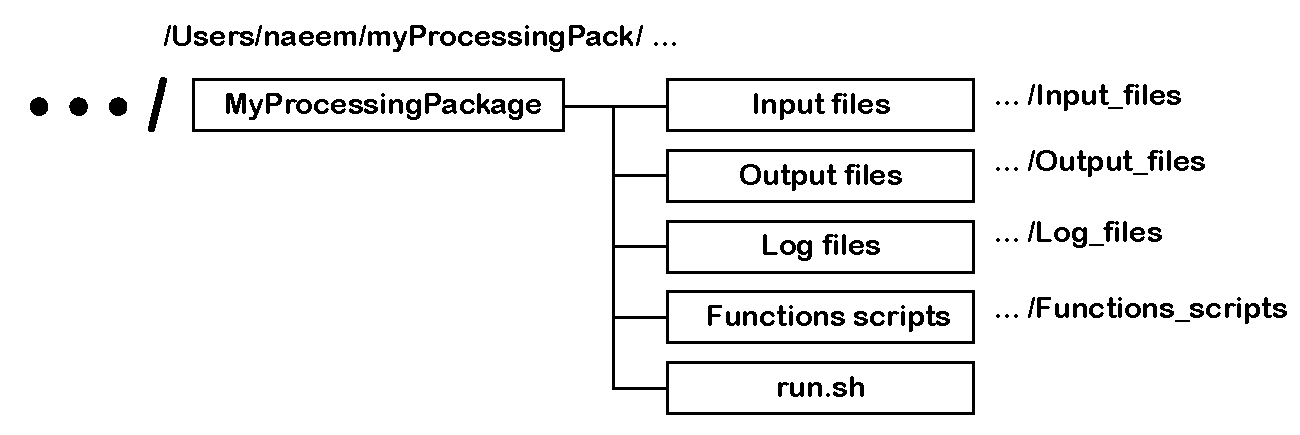
\includegraphics[scale=0.6]{figures/pdf/Figure03.pdf} 
\caption{Relative path of folders.}
\label{fig:structure}
\end{figure}

